\documentclass{article}
\usepackage[UTF8]{ctex}
\usepackage[T1]{fontenc}
\usepackage[utf8]{inputenc}
\usepackage{float}
\usepackage{placeins}
\usepackage{latexsym}
\usepackage{amsmath}
\usepackage{amsthm}
\usepackage{listings}
\usepackage{xcolor}


\title{Homework 2}
\author{PB17000297 罗晏宸}
\date{September 9 2019}

\begin{document}
\maketitle

\section{Exercise 2.3}
叙述由下列正规式描述的语言。\par
(d) $0^*\;10^*\;10^*\;10^*$\par
(e) $(00\ |\ 11)^*\;((01\ |\ 10)\;(00\ |\ 11)^*\;(01\ |\ 10)\;(00\ |\ 11)^*\;)^*$\par
并针对(e)给出识别相同正规集的极小化DFA。
\\

\paragraph{解}
\subparagraph{(d)}
正规式$0^*\;10^*\;10^*\;10^*$所描述的语言是字母表$\Sigma=\{0,\,1\}$上1的数量为3的所有串。
\subparagraph{(e)}
正规式$(00\ |\ 11)^*\;((01\ |\ 10)\;(00\ |\ 11)^*\;(01\ |\ 10)\;(00\ |\ 11)^*\;)^*$所描述的语言是字母表$\Sigma=\{0,\,1\}$上0和1的数量均为偶数的所有串。\par
对于$\Sigma=\{0,\,1\}$上任意一个输入串,依据串中0和1数量的奇偶性,可分为4种状态,DFA如下,
\begin{figure}
\centering
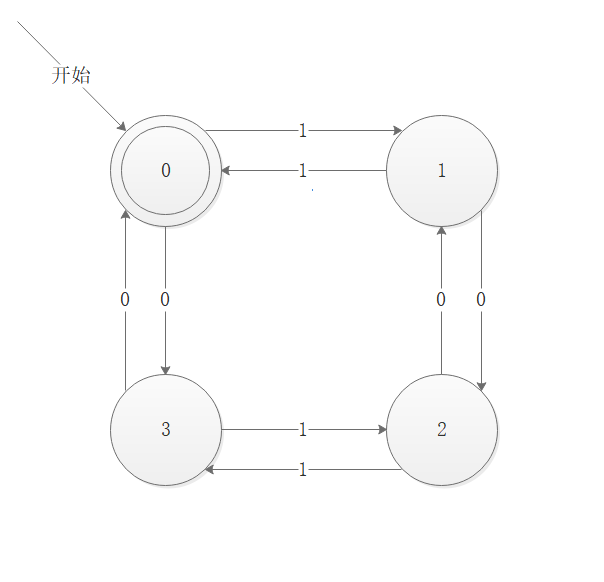
\includegraphics[scale=1]{DFA1.png}
\caption{接受0和1的数量均为偶数串的DFA}
\label{fig:1}
\end{figure}
其中:\par
状态0表示串中0和1的个数都为偶数;\par
状态1表示串中0的个数为偶数,1的个数为奇数;\par
状态2表示串中0和1的个数都为奇数;\par
状态3表示串中0的个数为奇数,1的个数为偶数.
\\

\section{Exercise 2.12}
为下列正规式构造最简的DFA。\par
(b) $(a\ |\ b)^*\;a\ (a\ |\ b)\;(a\ |\ b)$
\\

\paragraph{解}
此正规式表示字母表$\Sigma=\{a,\,b\}$上倒数第3个字符是a的所有串。由于最后两个字符的任意性,状态图应有4个接受状态,且状态图应从起始状态经两次分支到达接受状态,再补全a或b的转换,得:\par
\begin{figure}
\centering
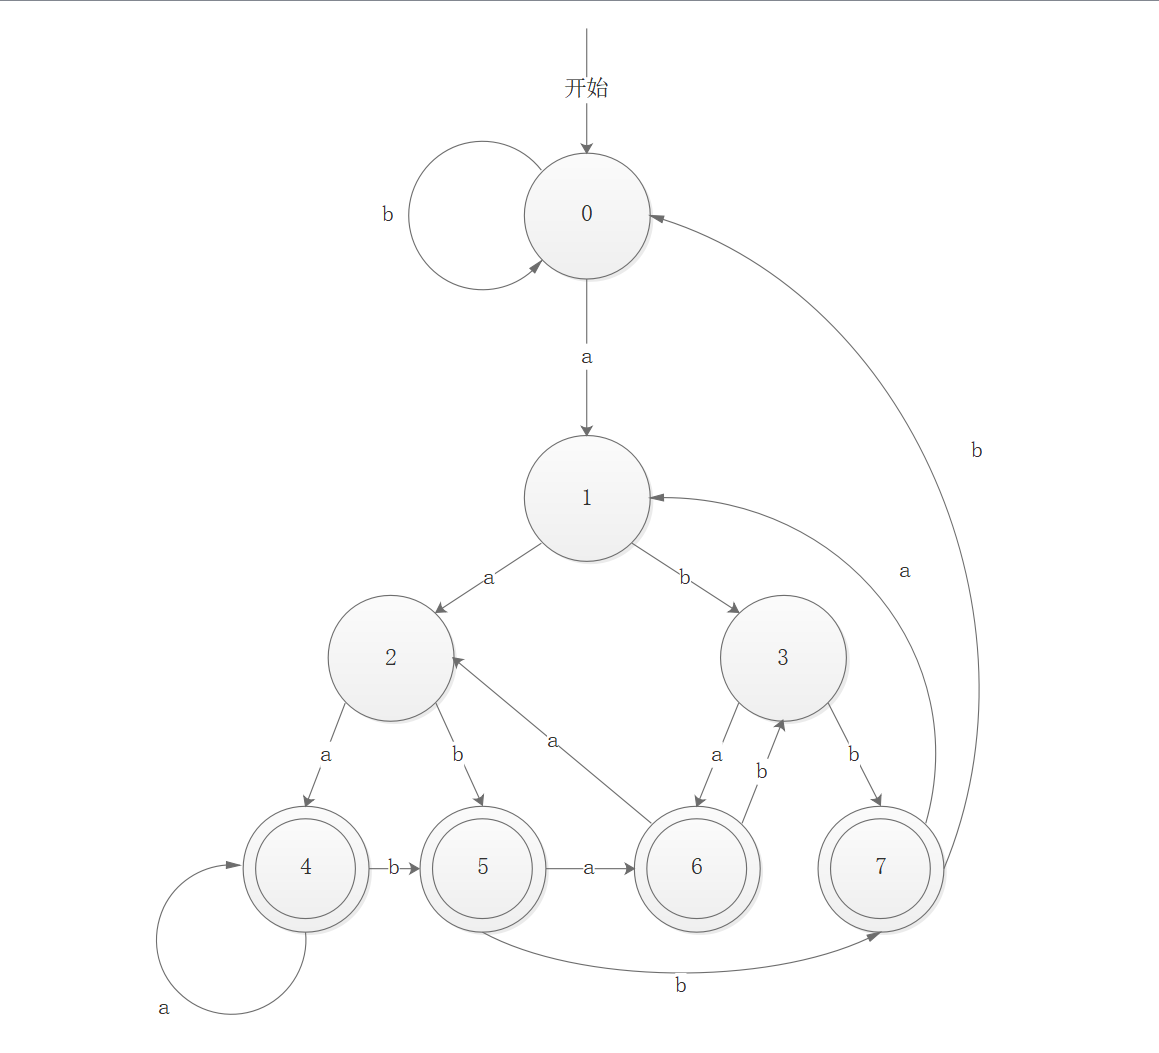
\includegraphics[scale=0.7]{DFA2.png}
\caption{接受倒数第3个字符是a的串的DFA}
\label{fig:2}
\end{figure}
下面进行简化。
\subparagraph{1}
初始划分$\Pi$:接受状态子集$F=\{4,\,5,\,6,\,7\}$,非接受状态子集$I=S-F=\{0,\,1,\,2,\,3\}$;
\subparagraph{2}
考查$I=\{0,\,1,\,2,\,3\}$:$0 \xrightarrow{a} 1$,$1 \xrightarrow{a} 2$,$2 \xrightarrow{a} 4$,$3 \xrightarrow{a} 6$,故将$I$划分成$I_1=\{0,\,1\}$和$I_2=\{2,\,3\}$。
考查$I_1=\{0,\,1\}$:$0 \xrightarrow{b} 0$,$1 \xrightarrow{b} 3$;考查$I_2=\{2,\,3\}$:$2 \xrightarrow{b} 5$,$3 \xrightarrow{b} 7$。
\subparagraph{3}
考查$F=\{4,\,5,\,6,\,7\}$:$4 \xrightarrow{a} 4$,$5 \xrightarrow{a} 6$,$6  \xrightarrow{a} 2$,$7 \xrightarrow{a} 1$,故将$F$划分成$F_1=\{4,\,5\}$和$F_2=\{6,\,7\}$。
考查$F_1=\{4,\,5\}$:$4 \xrightarrow{b} 5$,$5 \xrightarrow{b} 7$;考查$F_2=\{6,\,7\}$:$6 \xrightarrow{b} 3$,$7 \xrightarrow{b} 5$,故将$F_2$划分成$F_3=\{6\}$和$F_4=\{7\}$。
\subparagraph{4}
此时划分为$I_1$、$I_2$、$F_1$、$F_3$和$F_4$,即$\{0,\,1\}$、$\{2,\,3\}$、$\{4,\,5\}$、$\{6\}$和$\{7\}$。
考查$I_1=\{0,\,1\}$:$0 \xrightarrow{a} 1$,$1 \xrightarrow{a} 2$,故将$I_1$划分为$\{0\}$和$\{1\}$;
考查$I_2=\{2,\,3\}$:$2 \xrightarrow{a} 4$,$3 \xrightarrow{a} 6$,故将$I_2$划分为$\{2\}$和$\{3\}$;
考查$F_1=\{4,\,5\}$:$4 \xrightarrow{a} 4$,$5 \xrightarrow{a} 6$,故将$F_1$划分为$\{4\}$和$\{5\}$;\par
综上,前述DFA已为极小。
\\

\section{Exercise 2.14}
构造一个DFA,它接受$\Sigma=\{0,\,1\}$上能被5整除的二进制数。
并针对所得到DFA $M$,给出相应的正规式$R$,使得$L(R) = L(M)$。

\paragraph{解}
\\

\end{document}